\subsubsection{Comparing Data Sets and Files}
Comparing data sets is maybe the most important feature of this service. In doing this, a researcher can evaluate index values over time, using different data sets for different things. For example, a researcher may be working in a site, recording data in the morning and at night, every day for a week. The researcher would process both sets separately using whichever indices and parameters they wish, and name and tag the sets appropriately. Then, in the Results Catalog, they can select both data sets, and see visualizations comparing the two sets across time, to see how the index values match up on the same days but in the morning and at night.\par
From a research perspective, this is the best way to draw conclusions from the indices included in this service, as the more data that is collected and processed, the more sense they make. An example of this includes a forest where human interaction is on the rise. Using an index like ACI over time will help to make correlations as to how human invasion on the forest is affecting the bird population. Alternatively, for comparing across sites, if a species of bird is found in multiple locations, the ACI index can be used to roughly determine the number of these species in the area. Comparing this value across the sites is useful for determining species population in different areas.\\

\begin{center}
	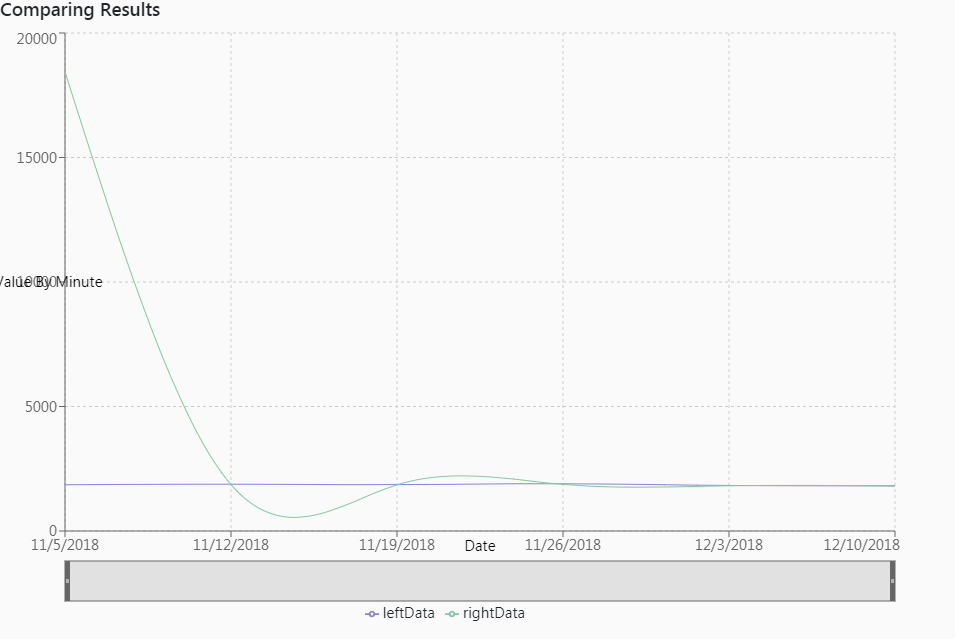
\includegraphics[width=\textwidth]{CompareACIgraph1} \\[12pt]
	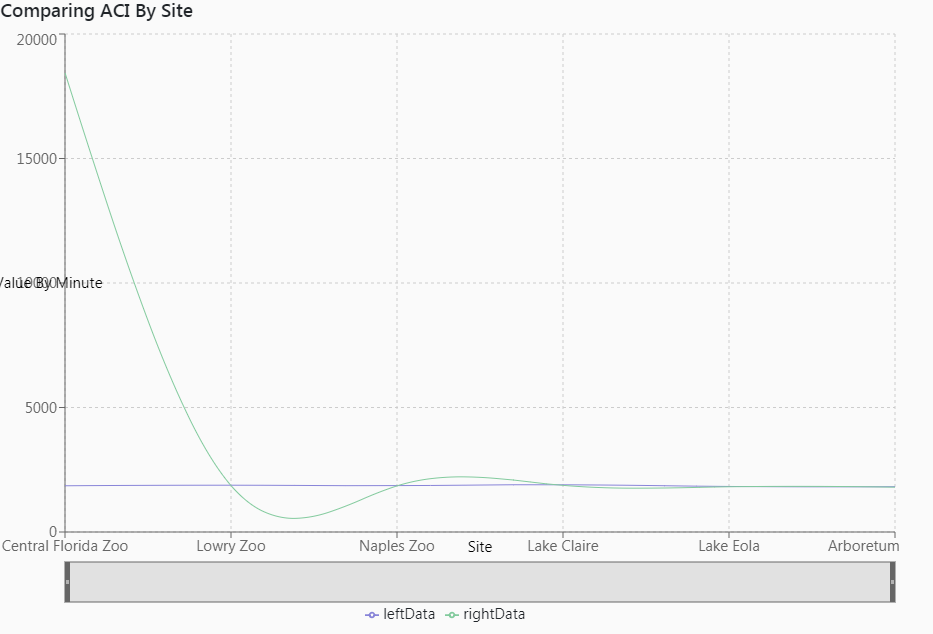
\includegraphics[width=\textwidth]{CompareACIgraph2} \\[12pt]
	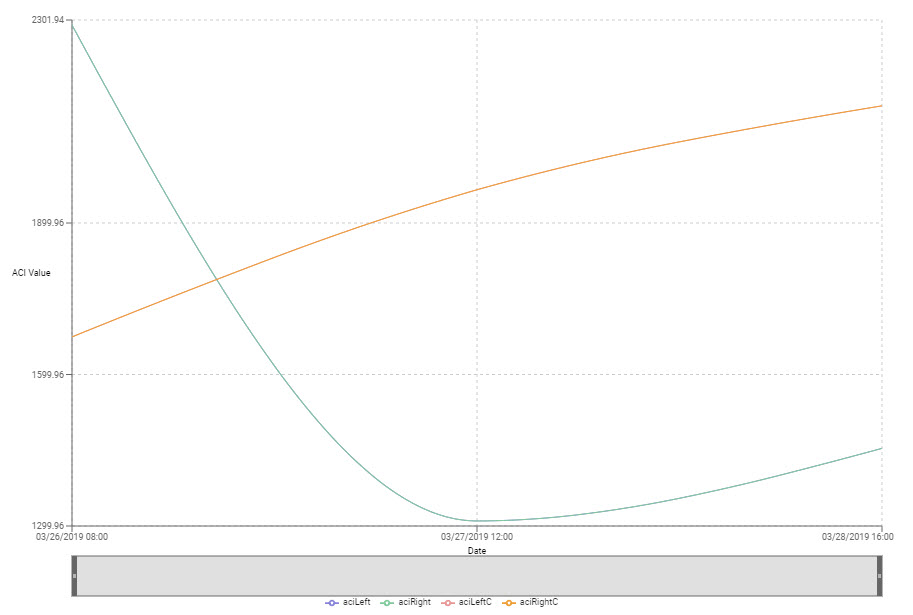
\includegraphics[width=\textwidth]{CompareACIgraph3} \\[12pt]
\end{center}

The first is a graph for comparing individual files in two different Sites or Sets. This graph shows you the ACI values over the recording time of each file. An audio player is available for this graph. The second graph is a file by file representation, allowing you to compare all the files in both sets of data being compared. This graph shows the overall ACI value of each file, rather than a time based approach. Finally, the last comparison graph for ACI is a comparison over date and time. This graph is a simple line graph with the overall ACI value by date and time being shown for both sets of data being compared.\\

\begin{center}
	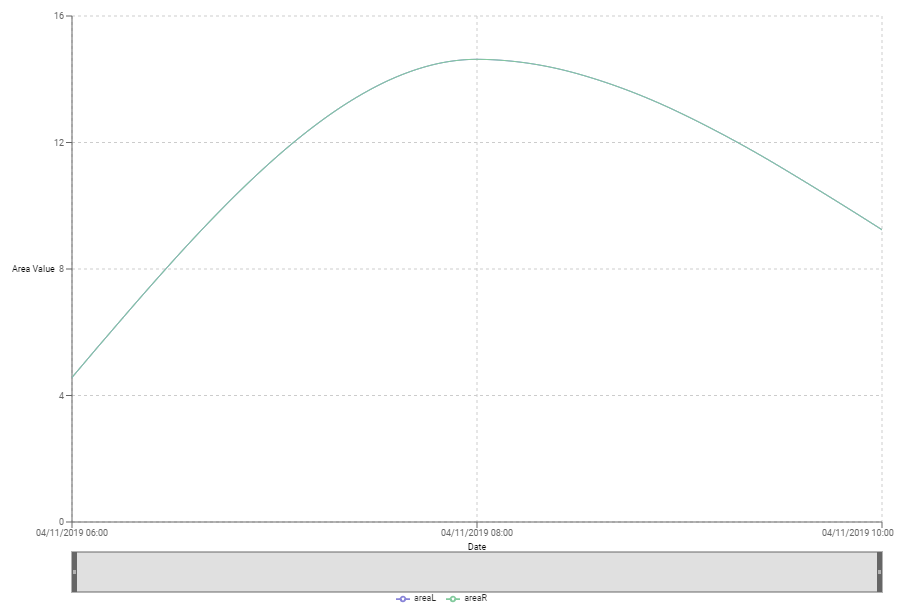
\includegraphics[width=\textwidth]{CompareBAgraph1} \\[12pt]
	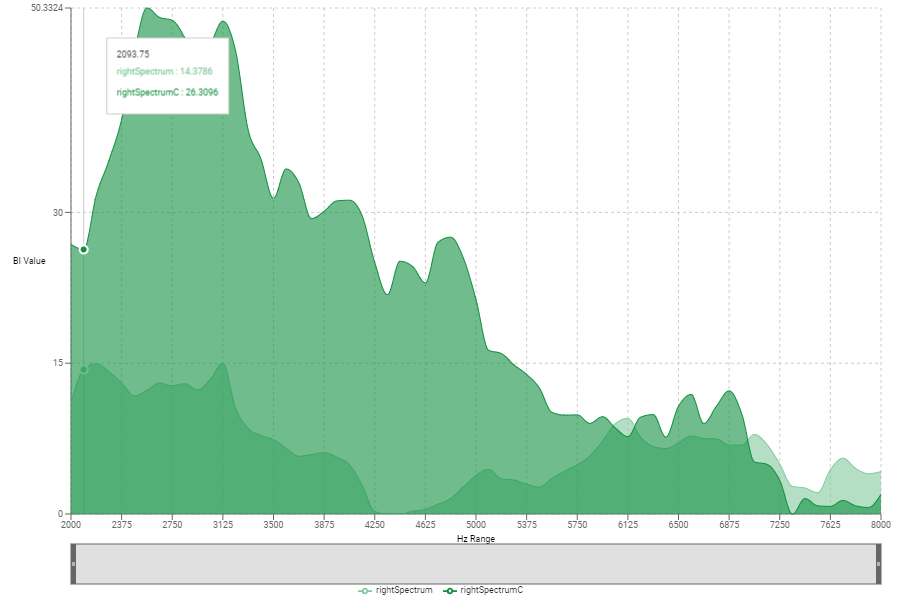
\includegraphics[width=\textwidth]{CompareBAgraph2} \\[12pt]
\end{center}

These two graphs represent the comparison charts available for the Bioacoustic Index. Again, the user has comparison across dates and research sites available to them. The brush is included to allow the user to shorten the observed time range as they please.\\

\begin{center}
	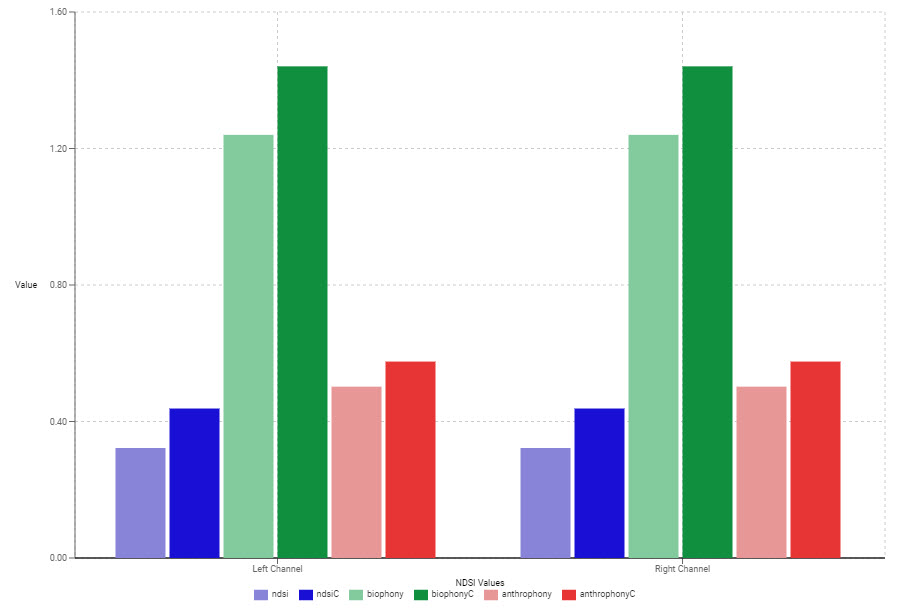
\includegraphics[width=\textwidth]{CompareNDSIgraph1} \\[12pt]
	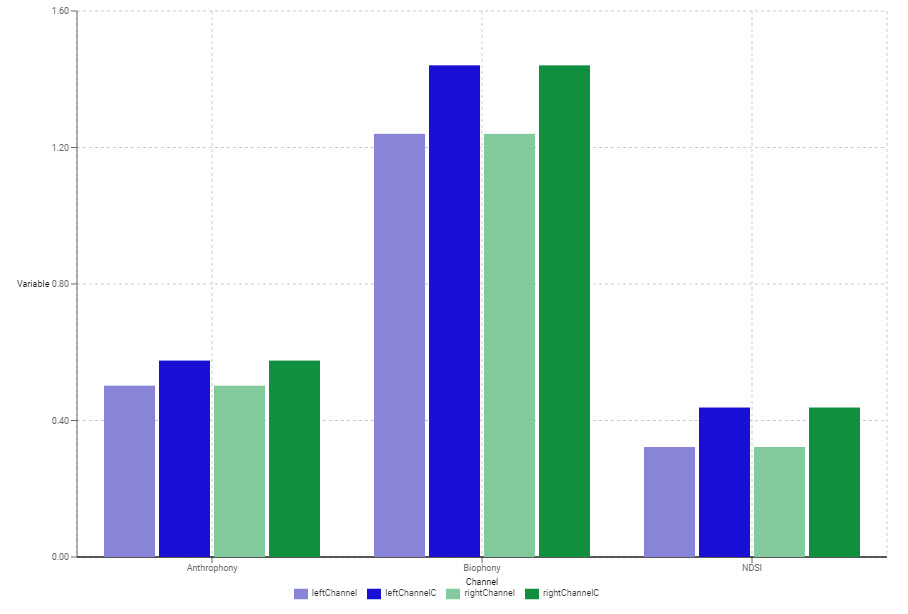
\includegraphics[width=\textwidth]{CompareNDSIgraph2} \\[12pt]
	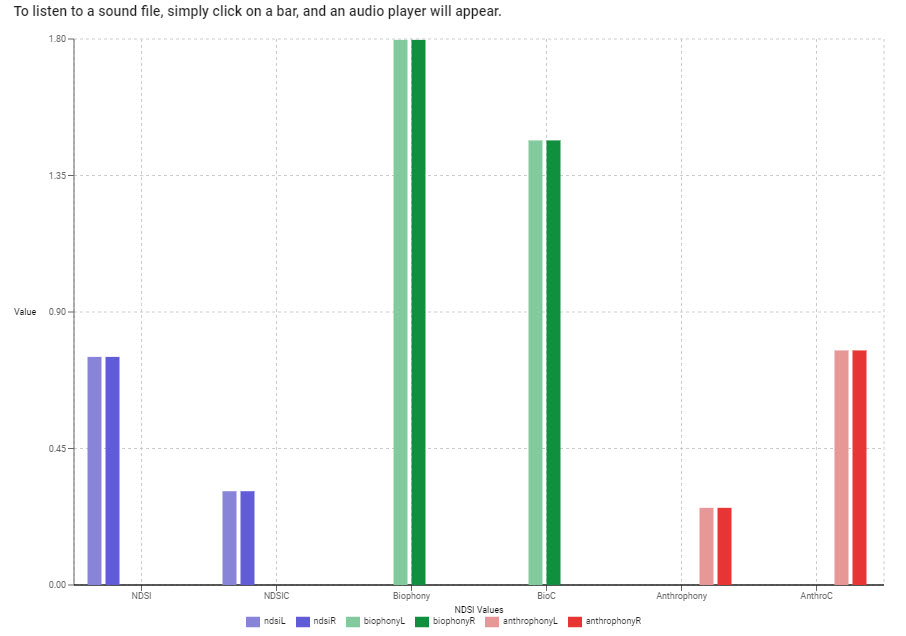
\includegraphics[width=\textwidth]{CompareNDSIgraph3} \\[12pt]
\end{center}

The comparison graphs for NDSI are much like the regular graphs. Here, additional bars are added to represent the data set being compared to as well. The first graph is the bar graph for comparing NDSI values by channel, while the second one is the bar graph for comparing channel NDSI values. The last graph is used to compare individual files in each data set being compared, and also allows for audio playback.\\

\begin{center}
	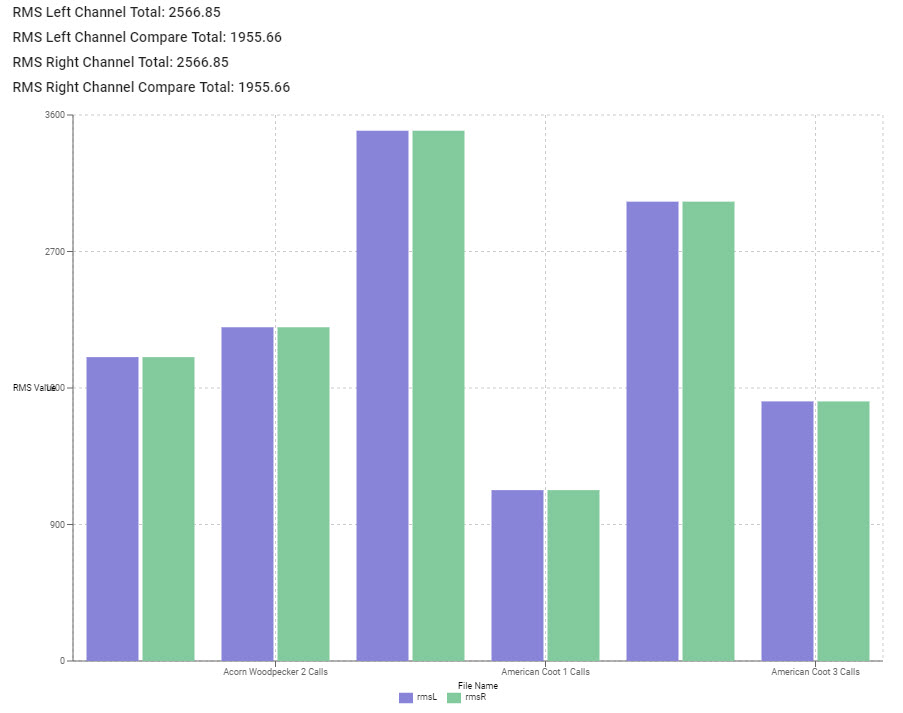
\includegraphics[width=\textwidth]{CompareRMSgraph1} \\[12pt]
\end{center}

Comparing RMS is fairly straight forward as RMS is simply a single value. The graph available includes a bar chart representing the RMS value for each file in the data being compared.
